\chapter{Bush ed Engelbart, Memex e Demo}

\section{Introduzione}

\dfn{Knowledge Navigator}{
    Un'idea di Apple, presentata nel 1987, di un assistente virtuale
    che aiuta l'utente a navigare tra le informazioni.
}

\subsubsection{Il filmato di presentazione del Knowledge Navigator (1987):}

\begin{itemize}
    \item [$\Rightarrow$] \fancyglitter{La comprensione del parlato}:
    il computer capisce il linguaggio naturale;
    \item [$\Rightarrow$] \fancyglitter{La grafica e le finestre}:
    dietro questo video c'è Alan Kay, che ha lavorato a Xerox PARC e fu 
    l'inventore delle finestre;
    \item [$\Rightarrow$] \fancyglitter{Il touch screen};
    \item [$\Rightarrow$] \fancyglitter{La videochiamata};
    \item [$\Rightarrow$] \fancyglitter{La simulazione}: della desertificazione.
\end{itemize}

\qs{}{Chi era Vannevar Bush?}

\paragraph{Risposta:} Vannevar Bush (1890 - 1974) era un ingegnere e scienziato americano.
Lui teorizzò il Memex
(non fu mai realizzato).

\nt{Durante una conferenza in occasione del 50° anniversario di "As 
we may think" (1945) venne presentata un'animazione del Memex.}

\section{Il Memex}

\dfn{Memex}{
    Un sistema di archiviazione e ricerca delle informazioni, teorizzato da Vannevar Bush.
}

\nt{Il Memex offre anche un'anticipazione di ciò che sarà l'\fancyglitter{
    ipertesto}, che nascerà vent'anni dopo.
}

\subsection{Problemi di organizzazione dell'informazione}

Il problema che preocupa Bush è \fancyglitter{la perdita di informazioni} che si accumula
continuamente nel tempo\footnote{Questo problema non era nuovo. 
Era già stato affrontato da Paul Otlet.}. Inoltre si aumenta progressivamente la
specializzazione: le informazioni sono sempre più frammentate e sempre più
specializzate (più difficili da comunicare). Bush ritiene che il problema 
non sia l'eccesso di pubblicazioni, ma il fatto che si siano estese oltre
la capacità di gestione dei documenti. 
La \fancyglitter{selezione}\footnote{Processo di scelta delle informazioni.}
è un problema per via delle enormi quantità di informazioni.

\ex{Addetto dell'ufficio informazioni}{
    L’addetto all’ufficio del personale di una fabbrica immette una pila di alcune migliaia di schede
degli impiegati in una macchina selezionatrice, imposta un codice secondo una convenzione
stabilita e produce in poco tempo una lista di tutti gli impiegati che vivono a Trenton e
conoscono lo spagnolo.
}

\ex{Centralini telefonici automatici}{
    Si compone un
numero e la macchina seleziona e connette solamente una tra un milione di possibili stazioni.
Non le ispeziona tutte. Presta attenzione solo a una classe data dalla prima cifra, poi solo a una
sottoclasse data dalla seconda cifra e così via; così procede rapidamente e quasi infallibilmente
verso la stazione selezionata.
}

\paragraph{Prroblemi di indicizzazione:}

\begin{itemize}
    \item [$\Rightarrow$] Si cerca da sottoclasse a sottoclasse;
    \item [$\Rightarrow$] L'informazione si trova in un unico punto (a meno che non sia duplicata);
    \item [$\Rightarrow$] Bisogna avere regole per specificare il percorso, ma le regole sono complicate;
    \item [$\Rightarrow$] Quando si trova l'elemento bisogna riemergere dal sistema e rientrare attraverso un nuovo percorso.
\end{itemize}

\nt{La situazione peggiore, ma più facilmente verificabile, è la ricerca in un albero.}

\dfn{Classificazione}{
    La \newfancyglitter{classificazione} è una segmentazione spaziale, temporale o spazio-temporale del mondo.
    
    Un sistema di classificazione è un insieme di scatole in cui si mettono cose per fare un 
    qualche tipo di lavoro.
}

\paragraph{Proprietà di un sistema di classificazione:}

\begin{itemize}
    \item [$\Rightarrow$] Ci sono principi univoci e consistenti;
    \item [$\Rightarrow$] Le categorie sono reciprocamente esclusive;
    \item [$\Rightarrow$] Il sistema è completo.
\end{itemize}
\pagebreak
\begin{figure}[h]
    \centering
    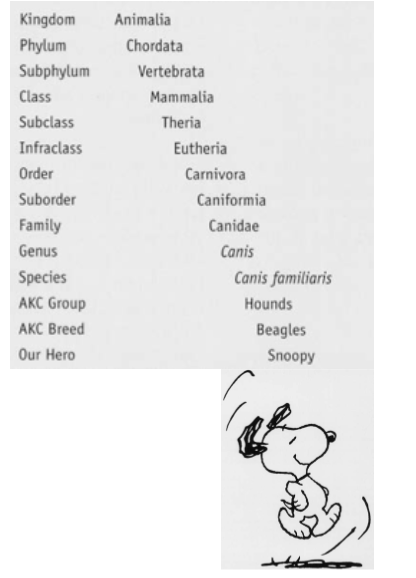
\includegraphics[scale=0.5]{images/Snoopy.png}
    \caption{Snoopy secondo due sistemi di classificazione.}
\end{figure}

\subsection{Indicizzazione}

\dfn{Indicizzazione}{
    L'\newfancyglitter{indicizzazione} è un'operazione è l'azione di descrivere o identificare
    un documento (o un oggetto) nei termini del suo contenuto concettuale\footnote{ISO 5963.}.
}

\nt{Lo scopo generale dell'indicizzazione è quello di rappresentare oggetti
in modo che possano essere efficacemente trovati e utilizzati.}

\cor{Linguaggio di indicizzazione}{
    Un linguaggio di indicizzazione è un sistema di rappresentazioni simboliche (un codice)
    che consentono la classificazione e la ricerca di documenti attraverso
    i codici assegnati ai concetti che essi contengono (indicizzazione per concetti).
}

\nt{Ted Nelson, in "As we may think", criticherà il fraintendimento
per cui si vede nel lavoro di Bush un contributo alla information retrieval\footnote{Reperimento di oggetti informativi.}.
}


\subsection{Browser vs Search}

Le seguenti definizioni sono state date da Clay Shirky in "Ontology is Overrated. 
Categories, Links, and Tags" (2005).

\dfn{Browse}{
    \newfancyglitter{Browse} significa che le persone fanno ontologia
    e categorizzazione, avendo la responsabilità di organizzare il mondo in anticipo.
}

\nt{Il browse è uno schema passivo.}

\dfn{Ricerca}{
    Il paradigma della \newfancyglitter{ricerca} sostiene che nessuno può
    prevedere cosa sarà necessario in futuro. Quando se ne ha bisogno si tenterà
    di trovarlo basandosi sulla struttura di link disponibile.
}

\nt{Per esempio, Google è un sistema di ricerca.}

\subsection{Associazione}

La mente umana, secondo Bush, lavora per associazione: quando 
"afferra" un elemento scatta istantanemente a quello successivo in base 
a un'associazione di pensieri in accordo con una rete di percorsi determinata dai neuroni.
La selezione per associazione può essere meccanizzata dal \fancyglitter{Memex}.

Nel Memex vengono archiviati tutti i libri, le registrazioni e le comunicazioni.
Esso è meccanizzato in modo da essere consultato con estrema velocità e flessibilità.
Si tratta di un supplemento \fancyglitter{personalizzato} ed allargato alla memoria dell'individuo.

\paragraph{Il Memex è uno strumento \textit{personale}:}

\begin{itemize}
    \item [$\Rightarrow$] È utilizzato da una sola persona;
    \item [$\Rightarrow$] L'utilizzatore lo adatta ai propri interessi;
    \item [$\Rightarrow$] Il Memex non è collegato ad altri dispositivi (non esiste una rete di Memex).
\end{itemize}

\nt{Il Memex è stato disegnato da Alfred D. Crimi, in Life.}

\clm{}{}{
    La versione del Memex su Life è stata letta da Engelbart in una 
    baracca della croce rossa in Filippine. Engelbart rievocherà
    questa descrizione tra la fine degli anni '50 e l'inizio degli anni '60
    quando deciderà di dedicarsi ad alcune problematiche di cui aveva avuto
    un'anticipazione nell'articolo di Bush.
}

\subsection{Le funzionalità del Memex}

La maggior parte dei contenuti del Memex è archiviata su microfilm (con rapid selector).
Il microfilm è un grande limite del Memex, in quanto analogico.

\paragraph{Le potenzialità del collegare elementi:}

\begin{itemize}
    \item [$\Rightarrow$] Fornisce un passo verso un'\fancyglitter{indicizzazione associativa}\footnote{Qualsiasi elemento può immediatamente selezionarne automaticamente un altro};
    \item [$\Rightarrow$] Quando un utente crea un percorso, il Memex lo \fancyglitter{nomina},
    \fancyglitter{inserisce il nome nel libro dei codici} e lo batte sulla tastiera;
    \item [$\Rightarrow$] In fondo a ogni elemento ci sono degli \fancyglitter{spazi vuoti} per immettere dei codici e viene impostato un puntatore per indicarne uno per ciascun elemento;
    \item [$\Rightarrow$] L'utente preme un singolo tasto e gli elementi vengono uniti in modo permanente\footnote{Nei relativi spazi appare il codice.}.
\end{itemize}

\subsubsection*{}
Questo processo fa si che, in qualsiasi momento, quando uno di questi elementi
viene richiamato, venga richiamato anche l'altro\footnote{Proprio come un ipertesto.}.
Si può dire che gli oggetti fisici siano stati raccolti da fonti remote e rilegati
insieme per \fancyglitter{formare un nuovo libro}\footnote{
    Quest'idea (un libro costruito attivamente da chi lo sta consultando), anticipata da Otlet,
    verrà ripresa da Licklider a proposito delle \fancyglitter{biblioteche del futuro}.
}.


\ex{Un Caso d'Uso del Memex}{
    \subsubsection{Questo esempio è ripreso parola per parola dalle slides del prof. Cardone.}

    Poniamo il caso che il proprietario del memex sia interessato all’origine e alle proprietà dell’arco
e delle frecce. Più precisamente egli sta studiando la ragione per cui l’arco corto turco fu
apparentemente migliore dell’arco lungo inglese nei combattimenti delle Crociate.

Egli ha dozzine di libri e articoli potenzialmente pertinenti nel suo memex.

Prima sfoglia un’enciclopedia, trova un articolo interessante ma non abbastanza dettagliato, e lo
lascia proiettato. Poi, in un libro di storia, trova un altro articolo pertinente e collega i due
insieme. Procede in questo modo, creando un percorso composto da molti elementi.

Occasionalmente inserisce un proprio commento, collegandolo al percorso principale o,
attraverso un percorso laterale, a uno specifico elemento.

Quando diventa evidente che le proprietà di elasticità dei materiali a disposizione avevano
molto a che fare con l’arco, egli crea una ramificazione su un percorso laterale che lo porta a testi
sull’elasticità e a tabelle di costanti fisiche.

Egli inserisce una pagina di analisi scritta a mano da lui stesso.

Quindi crea un percorso di suo interesse attraverso il labirinto dei materiali a sua disposizione.
Diversi anni più tardi [c]on un tocco accede al libro dei codici. Premendo alcuni tasti egli proietta
l’inizio del percorso. Con una leva lo scorre a piacere fermandosi sugli elementi interessanti,
facendo delle digressioni.

Appariranno tipi totalmente nuovi di enciclopedie, già munite di una rete di tracce associative
che le attraversano, pronte per essere immesse nel memex dove vengono ampliate. [Esempi
sull’uso di una grande massa di informazioni da parte di avvocati, medici e scienziati.]

Lo storico con un vasto resoconto cronologico di un popolo lo accosta ad un percorso saltuario
che si sofferma solamente sui temi salienti, e può seguire in ogni momento percorsi paralleli che
lo portano a spaccati di civiltà in particolari epoche.

}

\clm{}{}{
    Wikipedia è nata in un'ottica di collegamenti e di ipertesto. 
    Il concetto di \fancyglitter{wiki} è stato inventato da Ward Cunningham. 
    Il wiki è ispirato agli ipertesti e fu implementato per la prima volta in \fancyglitter{HyperCard}.
    Inoltre Cunningham è anche noto in ambito di programmazione OO per l'Extreme Programming (XP), visto nel corso 
    "Sviluppo Applicazioni Software".
}

\dfn{Apripista}{
    Un'\newfancyglitter{apripista} è una nuova professione che si occupa di
    stabilire \newfancyglitter{percorsi utili} attraverso l'enorme massa delle informazioni
    archiviate.
}

\section{Il progetto di Doug Engelbart: Demo}

\pagebreak

\begin{figure}
    \centering
    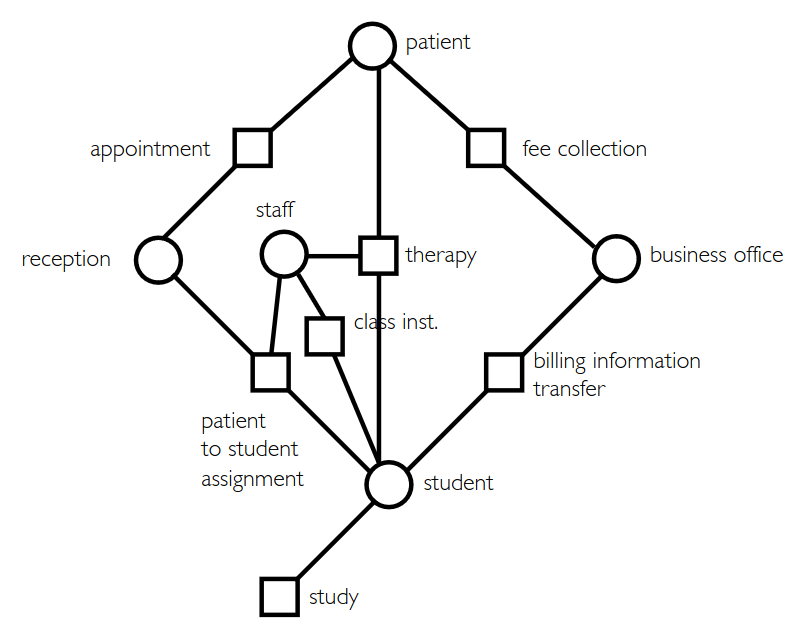
\includegraphics[scale=0.5]{images/UniBoston.png}
    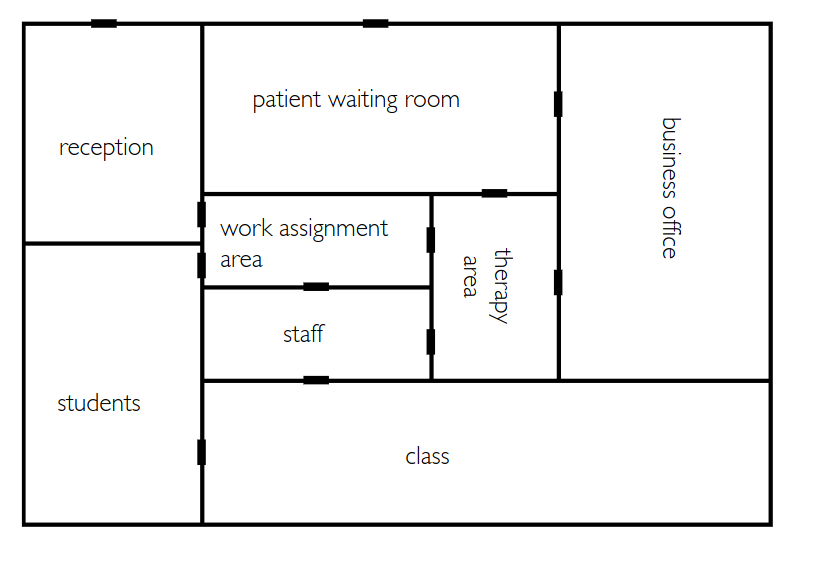
\includegraphics[scale=0.5]{images/UniBoston2.png}
    \caption{Il sistema di classificazione della scuola dentistica dell'Università di Boston.}
\end{figure}

\pagebreak

\begin{figure}
    \centering
    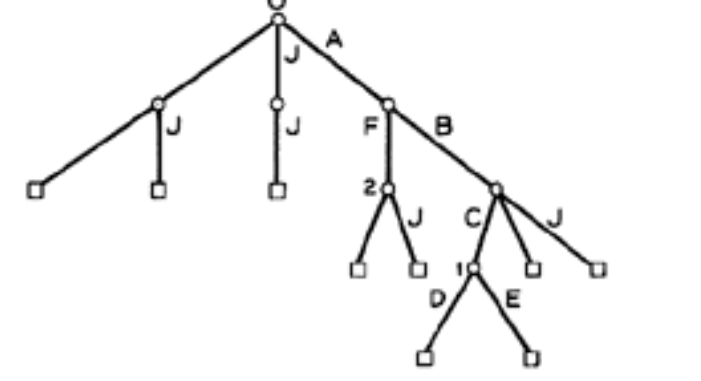
\includegraphics[scale=0.5]{images/Unix.png}
    \caption{Filesystem UNIX.}
\end{figure}

\begin{figure}
    \centering
    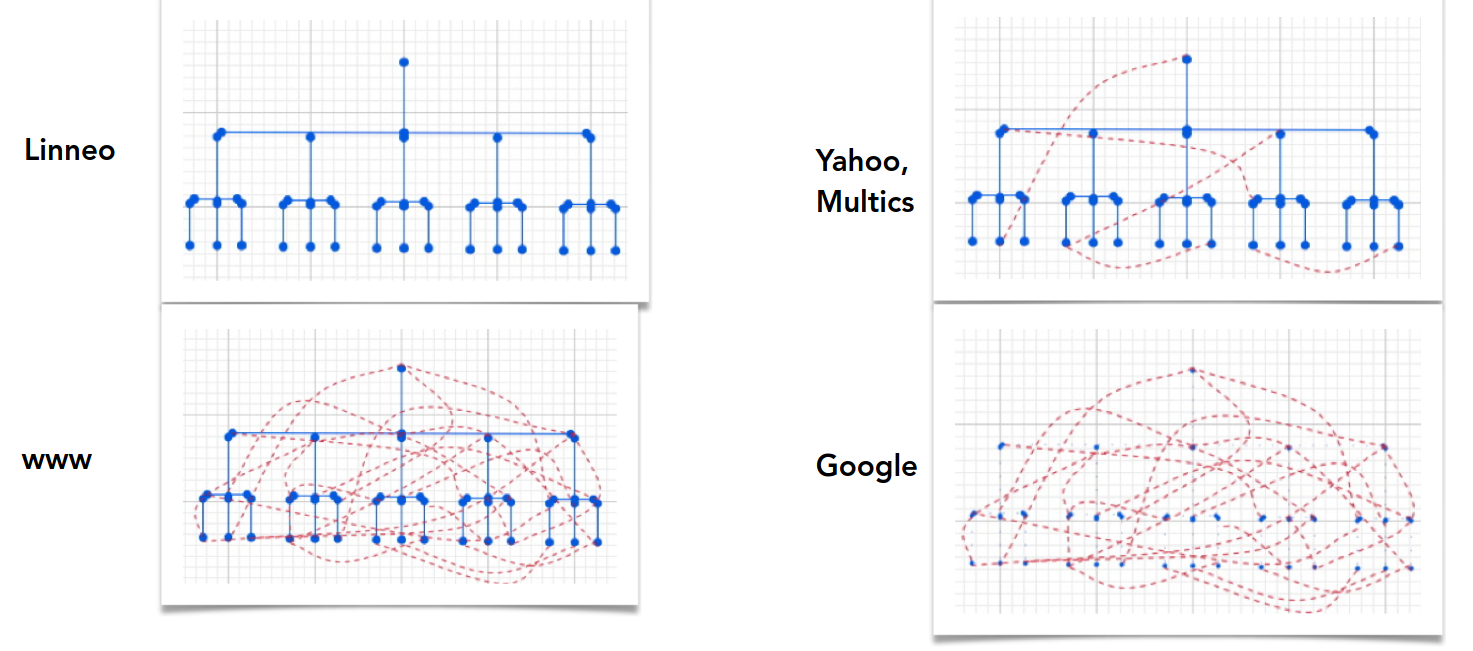
\includegraphics[scale=0.3]{images/C.png}
    \caption{Evoluzione delle gerarchie di classificazione.}
\end{figure}
